
\chapter{Encadenado de etapas dinámicas}\label{ch:ch3label}
\section{Introducción}
El inconveniente de la lógica dinámica es que no se pueden encadenar en cascado las etapas como sí se podría hacer con la lógica estática, sino que debemos procurar una buena conexión para que funcione.
\section{Esquemático del circuito}
En este apartado se ha dibujado otro banco de pruebas esta vez con dos BlockDyn encadenados entre sí:
\begin{figure}[h]%[!ht]
\begin {center}
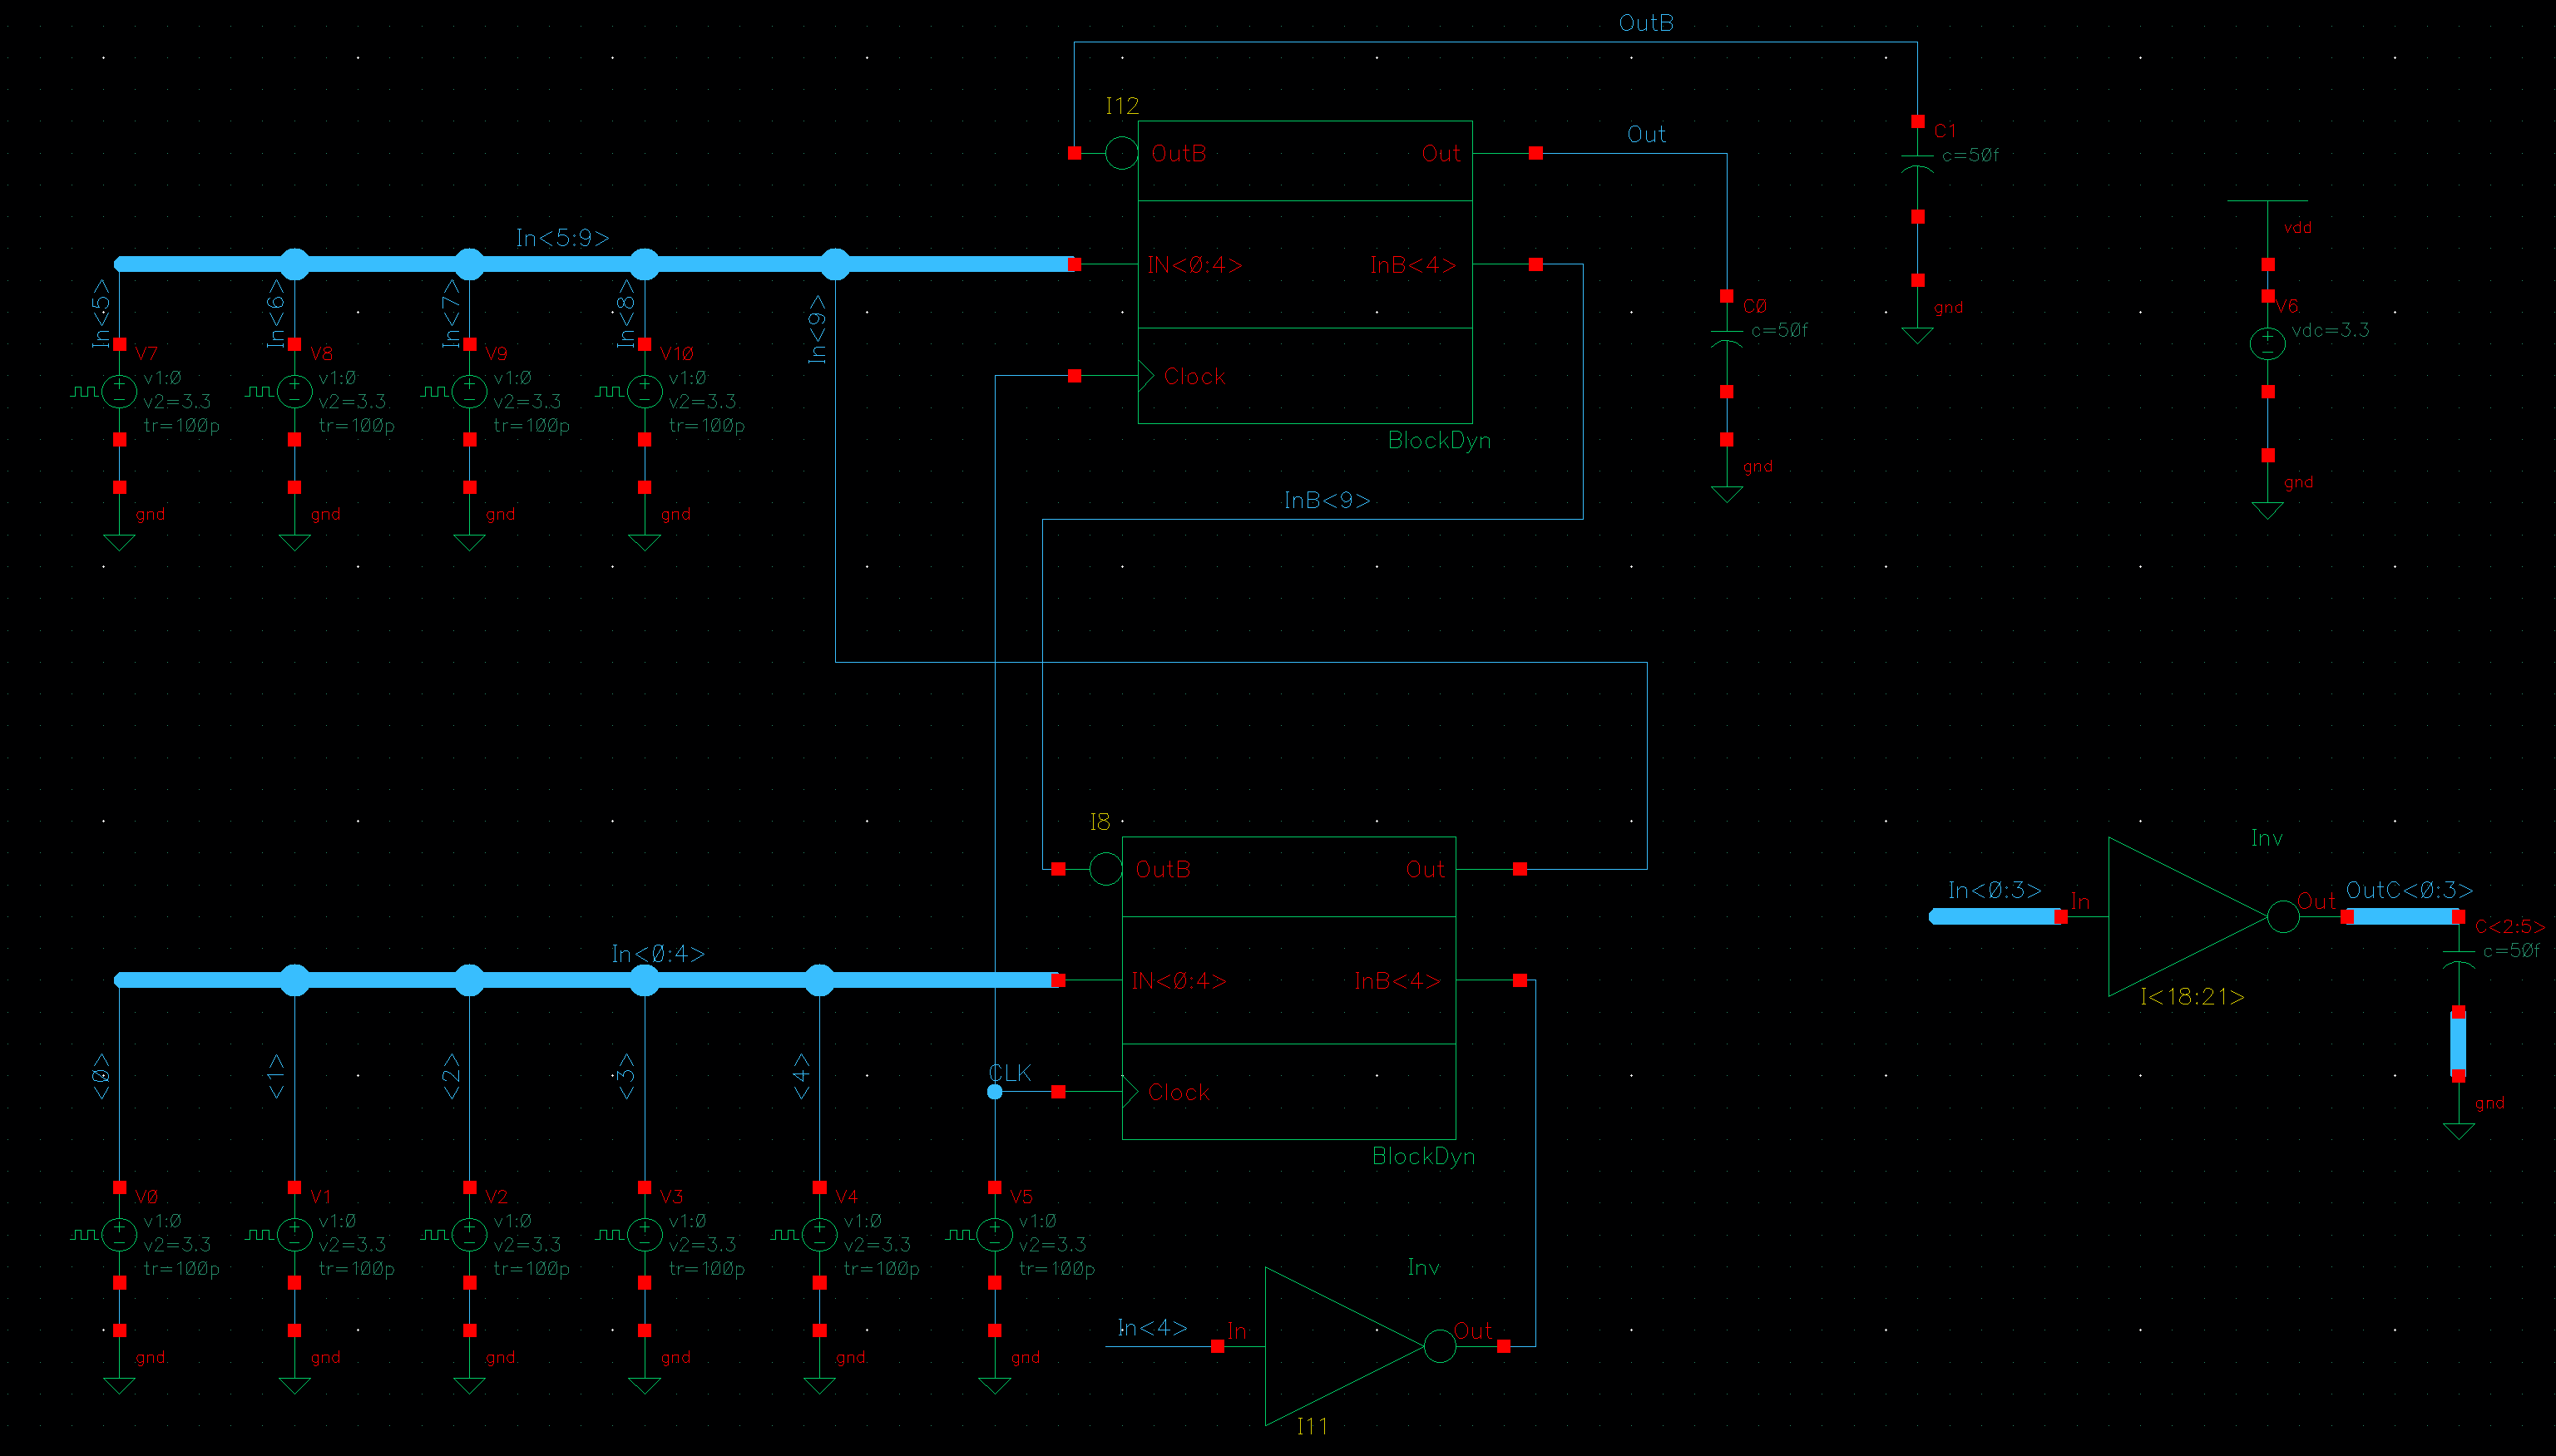
\includegraphics[width=1.1\textwidth]{figures/BlockDynEncTBSchem.PNG}
\caption{Banco de pruebas de 2 etapas BlockDyn correctamente encadenadas}
\label{fig:SchemTBEnc}
\end {center}
\end{figure} \newline
Apréciense la forma especial en la que se deben conectar los 2 bloques, siempre la salida del anterior al último bit de entrada de la siguiente, nunca a ningún otro. Se hará una simulación para ver qué pasa en caso de no cumplirse esta afirmación. \newgeometry{top=3cm, bottom=2cm}
\section{Análisis transitorio}
\par En primer lugar, se ha creado un estado nuevo con una frecuencia de 200MHz y un tiempo de simulación de 1.5u para ver todas las combinaciones posibles:
\begin{figure}[h]%[!ht]
\begin {center}
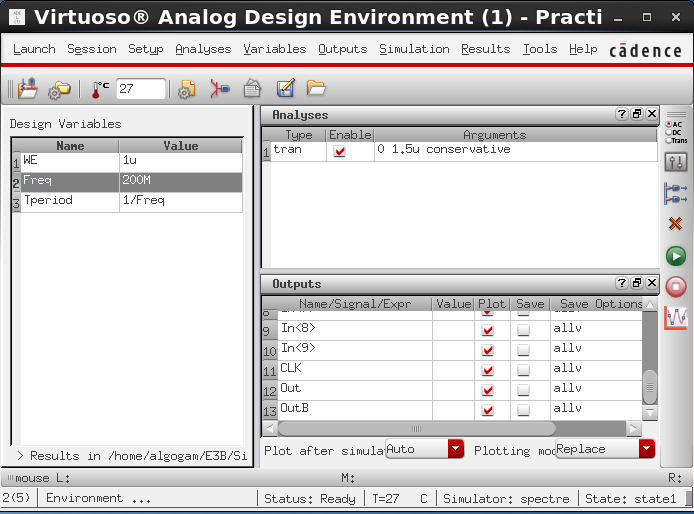
\includegraphics[width=0.7\textwidth]{figures/StateEncConfig.PNG}
\caption{Configuración del ADE para el banco de pruebas del encadenado}
\label{fig:ConfigTBEnc}
\end {center}
\end{figure} \newline
Sin embargo, en la captura que aquí se muestra, se ha hecho un zoom a los primeros 400ns para tener una mejor visión de las salidas, ya que estás aparecían demasiado estrechas si se tomaba una captura del tiempo de simulación completo:
\begin{figure}[H]%[!ht]
\begin {center}
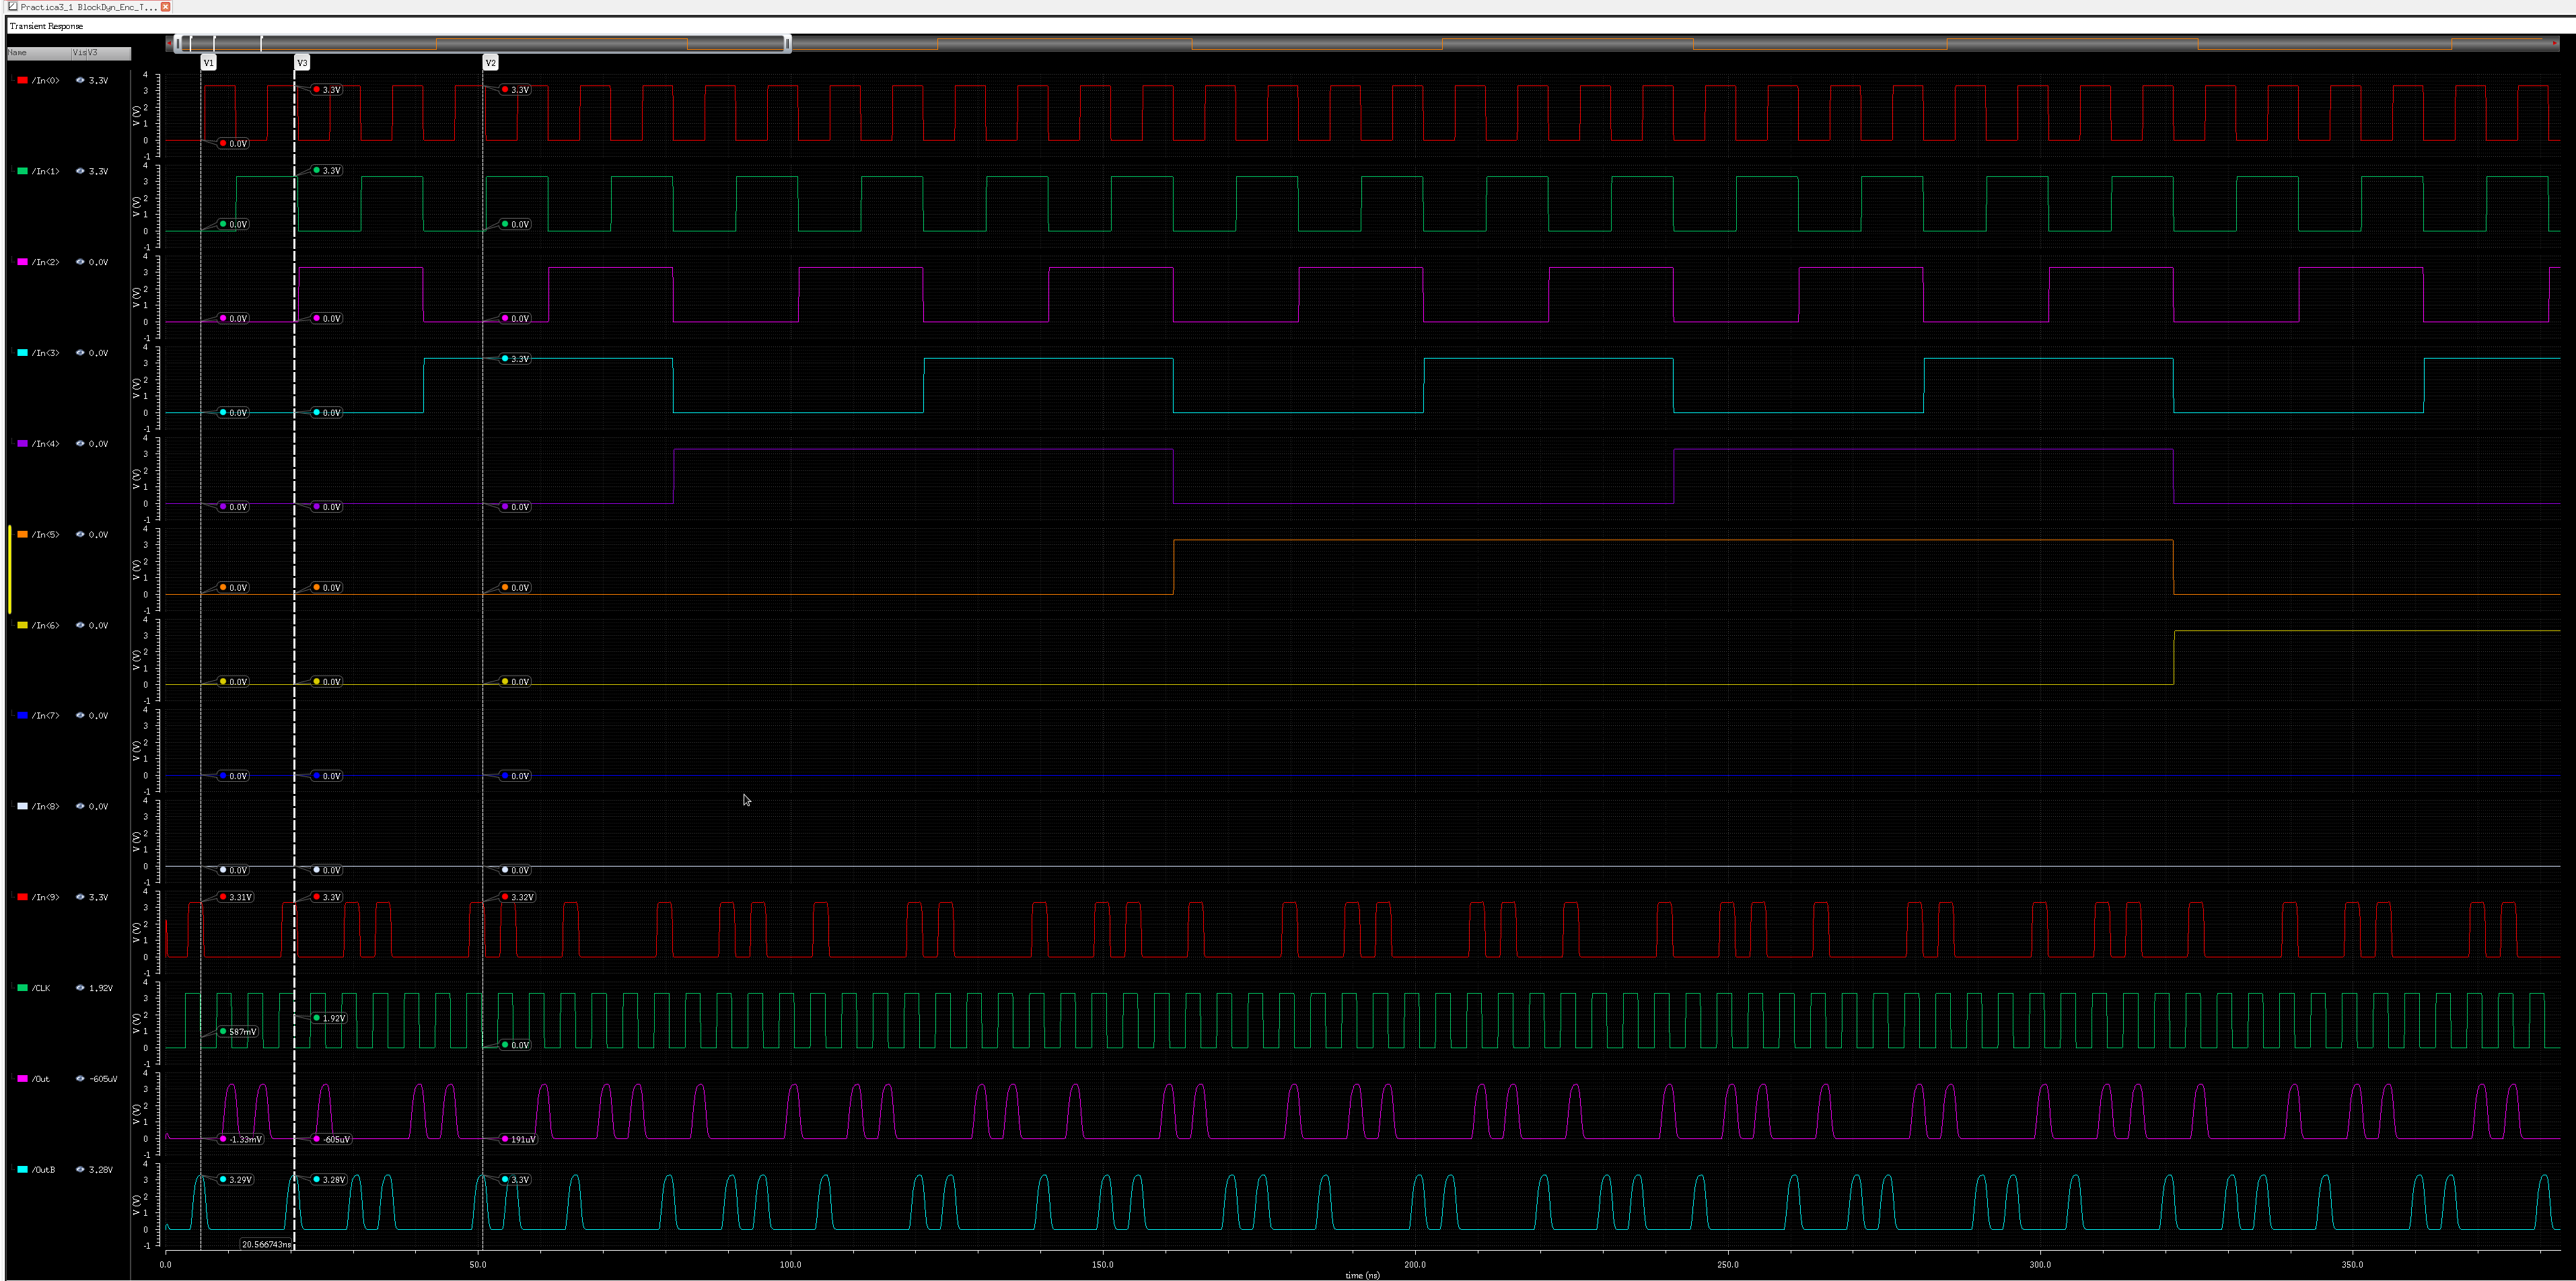
\includegraphics[width=1\textwidth]{figures/GraphEncTB.png}
\caption{Gráfica del banco de pruebas del Encadenado de Etapas Dinámicas}
\label{fig:GraphTBEnc}
\end {center}
\end{figure}
Como se puede observar, la función lógica la hace, de forma correcta, tomando la entrada In<9> como la salida de la primera etapa.  \newpage Tanto la salida Out como su negada OutB son correctas. La forma que presentan (un pulso con un tiempo de subida apreciable) se debe al retardo de propagación que hace que la salida tarde más en alcanzar el nivel alto. La salida de la primera etapa In<9> no presenta este problema ya que obtiene el resultado antes que la segunda etapa, consecuencia de que estemos empleando lógica dominó (las siguientes etapas no se actualizan hasta que no lo han hecho las primeras).

Ahora bien, ¿qué pasaría si encadenáramos mal las etapas y conectáramos la salida de la primera etapa a otra entrada de la segunda? Nos hemos tomado la libertad de simular este caso, cambiando la conexión \say{by name} de la siguiente manera:
\begin{figure}[H]%[!ht]
\begin {center}
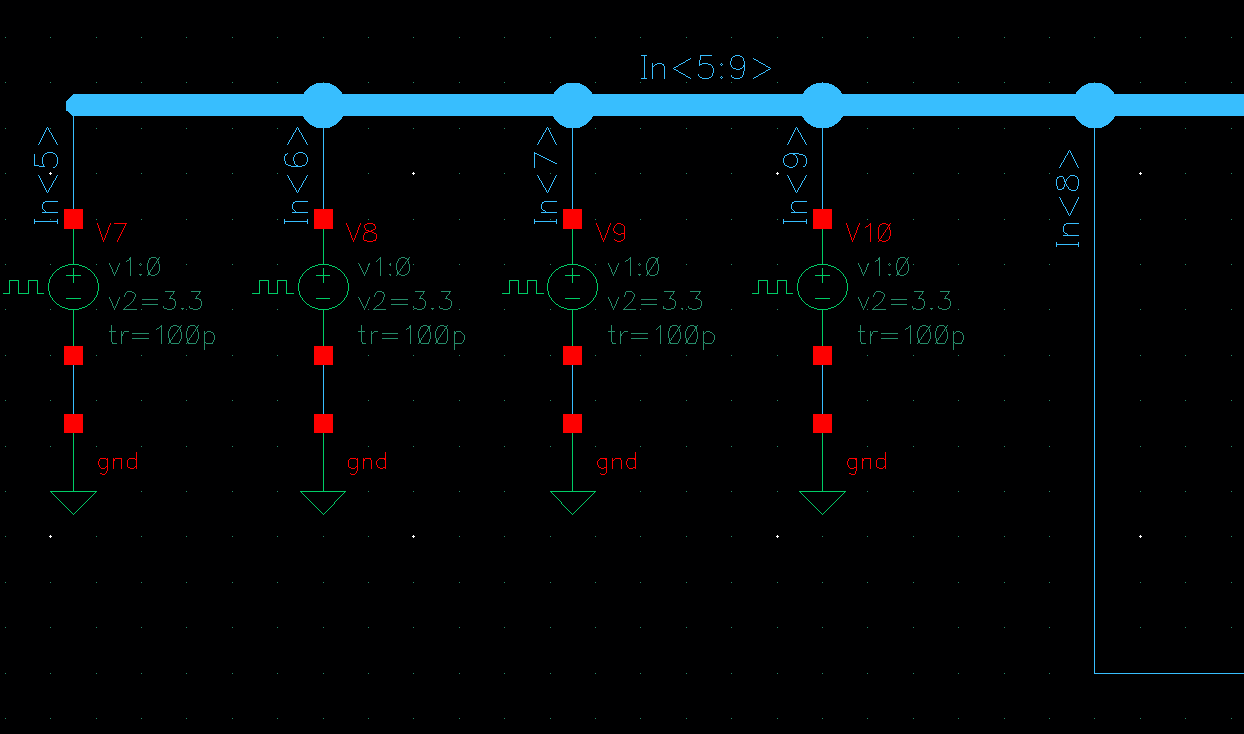
\includegraphics[width=0.75\textwidth]{figures/BlockDynBadSchem.PNG}
\caption{Detalle de la mala conexión de una etapa dinámica con la siguiente}
\label{fig:SchemBadEnc}
\end {center}
\end{figure}
Donde se ha intercambiado la etiqueta In<9> con la etiqueta In<8>. Corriendo una simulación en estas circunstancias, se obtuvo lo siguiente:
\begin{figure}[H]%[!ht]
\hspace{-10mm}
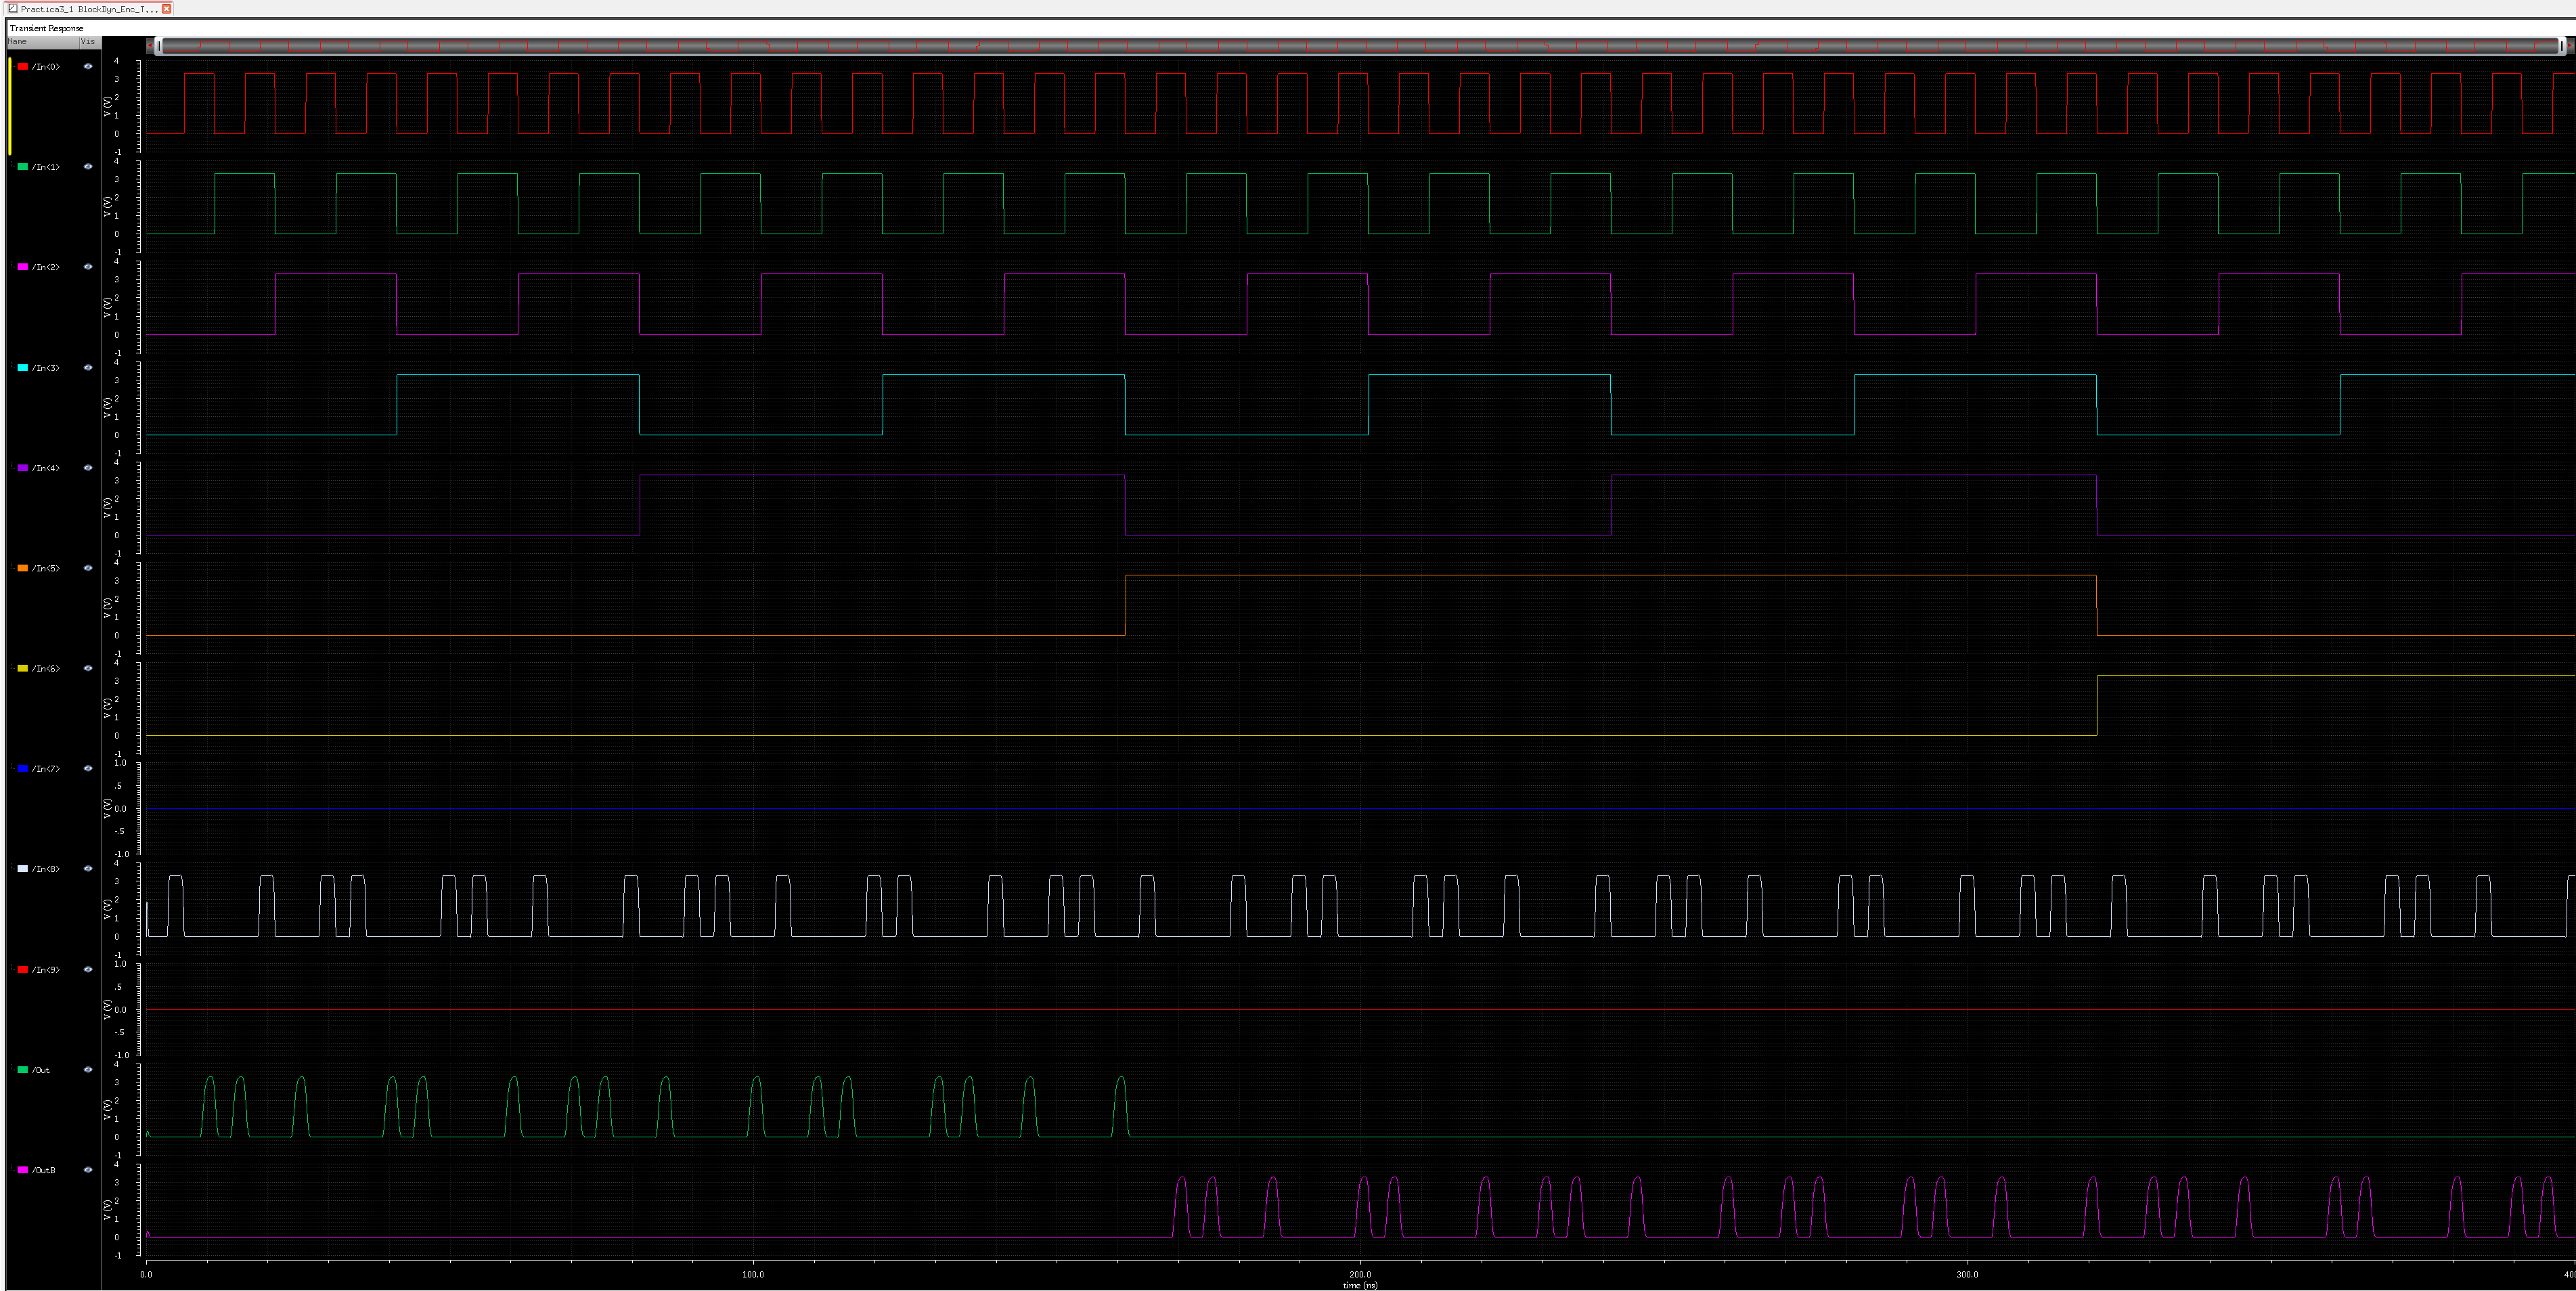
\includegraphics[width=1.2\textwidth]{figures/GraphEncBad.png}
\caption{Simulación de un banco de pruebas con etapas dinámicas incorrectamente encadenadas}
\label{fig:GraphBadEnc}

\end{figure}

Basta con comparar las trazas de Out y OutB para ver que algo no va bien: la salida de OutB no es la negada de Out y, otro comportamiento a tener en cuenta es que sólo una de las dos señales permanece en funcionamiento al mismo tiempo, es decir, en los primeros instantes de la simulación, OutB no muestra signos de ponerse a nivel alto y se queda todo el rato a cero, a pesar de que hay instantes, como se ha visto en la figura \ref{fig:GraphTBEnc}, en los que se debería poner a nivel alto. En conclusión, se hace necesaria la conexión de la forma que se indica en el guion de la práctica. La razón por la que no se podían conectar etapas dinámicas de forma directa era que el retardo de propagación para descargar el primer nodo de salida puede provocar una descarga no deseada de la salida de la siguiente puerta, lo que resulta en una degradación a niveles lógicos. Aquí vemos que hay una degradación que se sigue produciendo en una de las dos salidas.

\restoregeometry

